\documentclass{article}
\usepackage{amsmath}
\usepackage{amsfonts}
\usepackage{amssymb}
\usepackage{geometry}
\usepackage{graphicx}
\usepackage{placeins}
\usepackage{flafter}
\usepackage{xcolor}
\usepackage{listings}
\usepackage[affil-it]{authblk}
\geometry{a4paper, margin=1in}

\title{Algorithmic Methods for Mathematical Models\\
 Course Project}
\author{Marco Bartoli, Ilan Vezmarovic \\
    UPC Universitat Politècnica de Catalunya}

\begin{document}

\maketitle

\section{Formal Problem Definition}

\subsection{Inputs}

\begin{itemize}
    \item $n$: number of products
    \item $x$: height of the suitcase in millimeters
    \item $y$: width of the suitcase in millimeters
    \item $c$: limit to the total weight of the suitcase in grams
    \item $p_i$: price of the $i$-th product in euros
    \item $w_i$: weight of the $i$-th product in grams
    \item $s_i$: side length of the $i$-th product's (square) box in millimeters
\end{itemize}

\subsection{Outputs}

\begin{itemize}
    \item Indices of the products chosen to maximize the accumulated price
    \item Arrangement of the products in the suitcase
\end{itemize}

\section{Mathematical Formulation}

\subsection{Decision Variables}

\begin{itemize}
    \item $\text{Chosen}_i$: binary variable that is 1 if object $i$ is chosen, and 0 otherwise.
    \item $\text{PointsX}_i$: the x-coordinate of the bottom-left corner of object $i$.
    \item $\text{PointsY}_i$: the y-coordinate of the bottom-left corner of object $i$.
    \item $\text{Overlap}_{i,j,d}$: binary variable indicating if objects $i$ and $j$ do not overlap in direction $d$, where $d \in \{1, 2, 3, 4\}$.
\end{itemize}

\subsection{Objective Function}

Maximize the total price of the chosen objects:

\[
\text{maximize} \sum_{i=1}^n p_i \cdot \text{Chosen}_i
\]

\subsection{Constraints}

\subsubsection{Max Weight Constraint}

Ensure the total weight of the chosen objects does not exceed the suitcase's capacity:

\[
\sum_{i=1}^n w_i \cdot \text{Chosen}_i \leq c
\]

\subsubsection{Coordinate Bounds Constraints}

Ensure each object lies entirely within the suitcase's boundaries:

\[
\forall i \in \{1, \ldots, n\}, \quad \text{PointsX}_i \geq 1
\]

\[
\forall i \in \{1, \ldots, n\}, \quad \text{PointsY}_i \geq 1
\]

\[
\forall i \in \{1, \ldots, n\}, \quad \text{PointsX}_i + s_i - 1 \leq x
\]

\[
\forall i \in \{1, \ldots, n\}, \quad \text{PointsY}_i + s_i - 1 \leq y
\]

\subsubsection{Non-Overlapping Constraints}

Ensure no two chosen objects overlap within the suitcase using the big-M method:

1. Horizontal non-overlapping to the right:

\[
\forall i, j \in \{1, \ldots, n\}, i \neq j, \quad \text{PointsX}_i - \text{PointsX}_j + s_i \leq -M \cdot (\text{Chosen}_i + \text{Chosen}_j + \text{Overlap}_{i,j,1} - 3)
\]

2. Horizontal non-overlapping to the left:

\[
\forall i, j \in \{1, \ldots, n\}, i \neq j, \quad \text{PointsX}_j - \text{PointsX}_i + s_j \leq -M \cdot (\text{Chosen}_i + \text{Chosen}_j + \text{Overlap}_{i,j,2} - 3)
\]

3. Vertical non-overlapping upwards:

\[
\forall i, j \in \{1, \ldots, n\}, i \neq j, \quad \text{PointsY}_i - \text{PointsY}_j + s_i \leq -M \cdot (\text{Chosen}_i + \text{Chosen}_j + \text{Overlap}_{i,j,3} - 3)
\]

4. Vertical non-overlapping downwards:

\[
\forall i, j \in \{1, \ldots, n\}, i \neq j, \quad \text{PointsY}_j - \text{PointsY}_i + s_j \leq -M \cdot (\text{Chosen}_i + \text{Chosen}_j + \text{Overlap}_{i,j,4} - 3)
\]

\subsubsection{At Least One Not Overlapping Constraint}

Ensure that for any two objects, at least one of the non-overlapping conditions is satisfied:

\[
\forall i, j \in \{1, \ldots, n\}, i \neq j, \quad \sum_{d=1}^4 \text{Overlap}_{i,j,d} \geq 1
\]

\newpage

\section{Tuning Local Search}

\begin{figure}[!h]
    \centering
    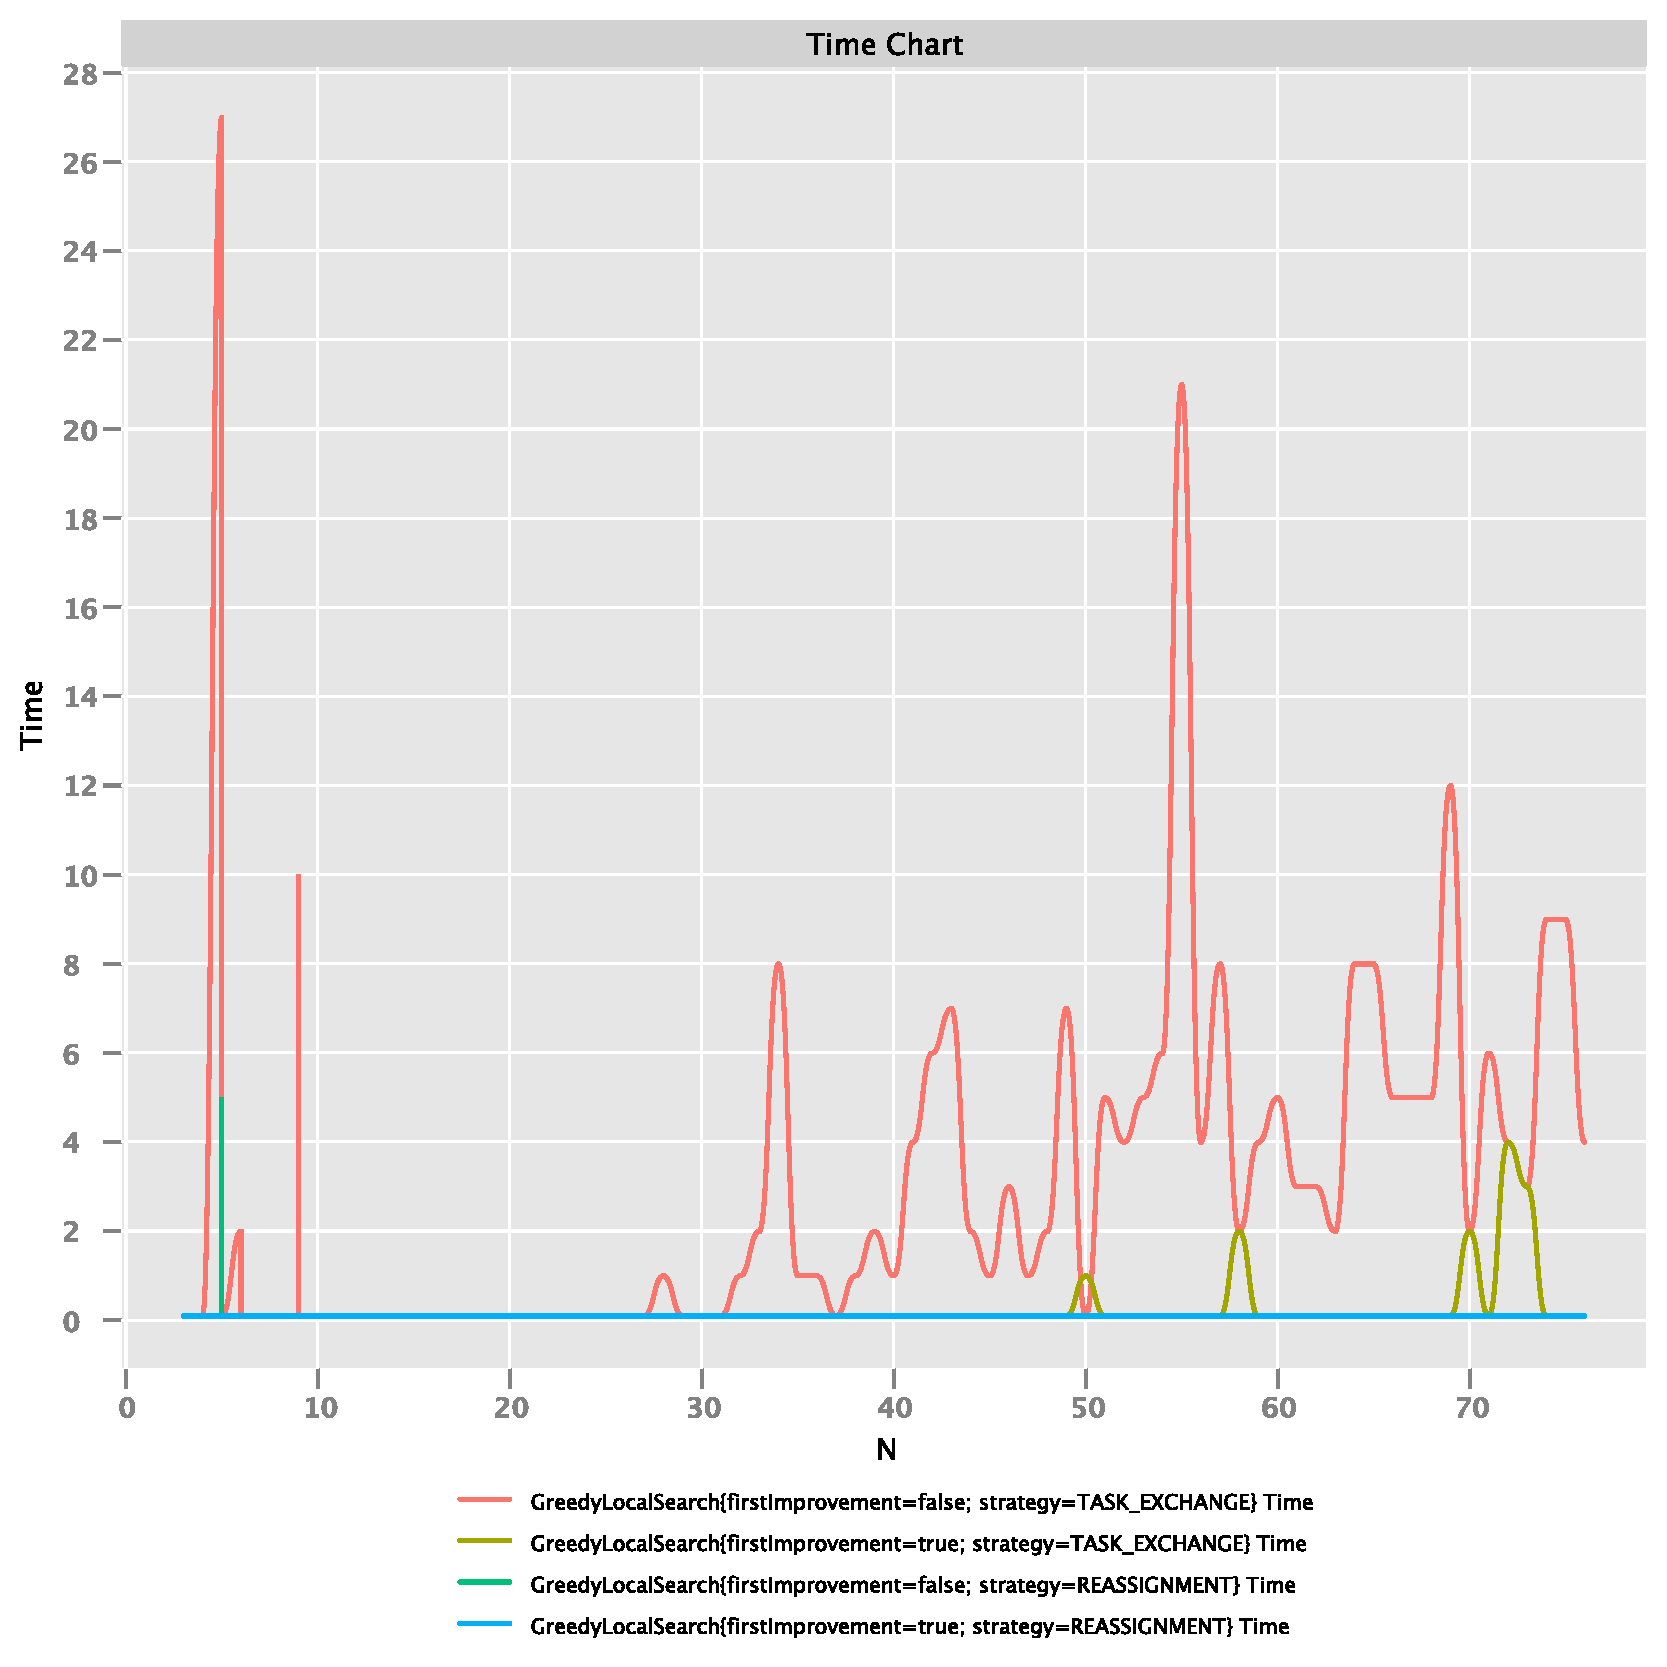
\includegraphics[width=0.9\textwidth]{./documentation/assets/localSearchParams.timeChart.pdf}
    \caption{Time Parameters Local Search}
    \label{fig:local_time}
\end{figure}\FloatBarrier

\begin{figure}
    \centering
    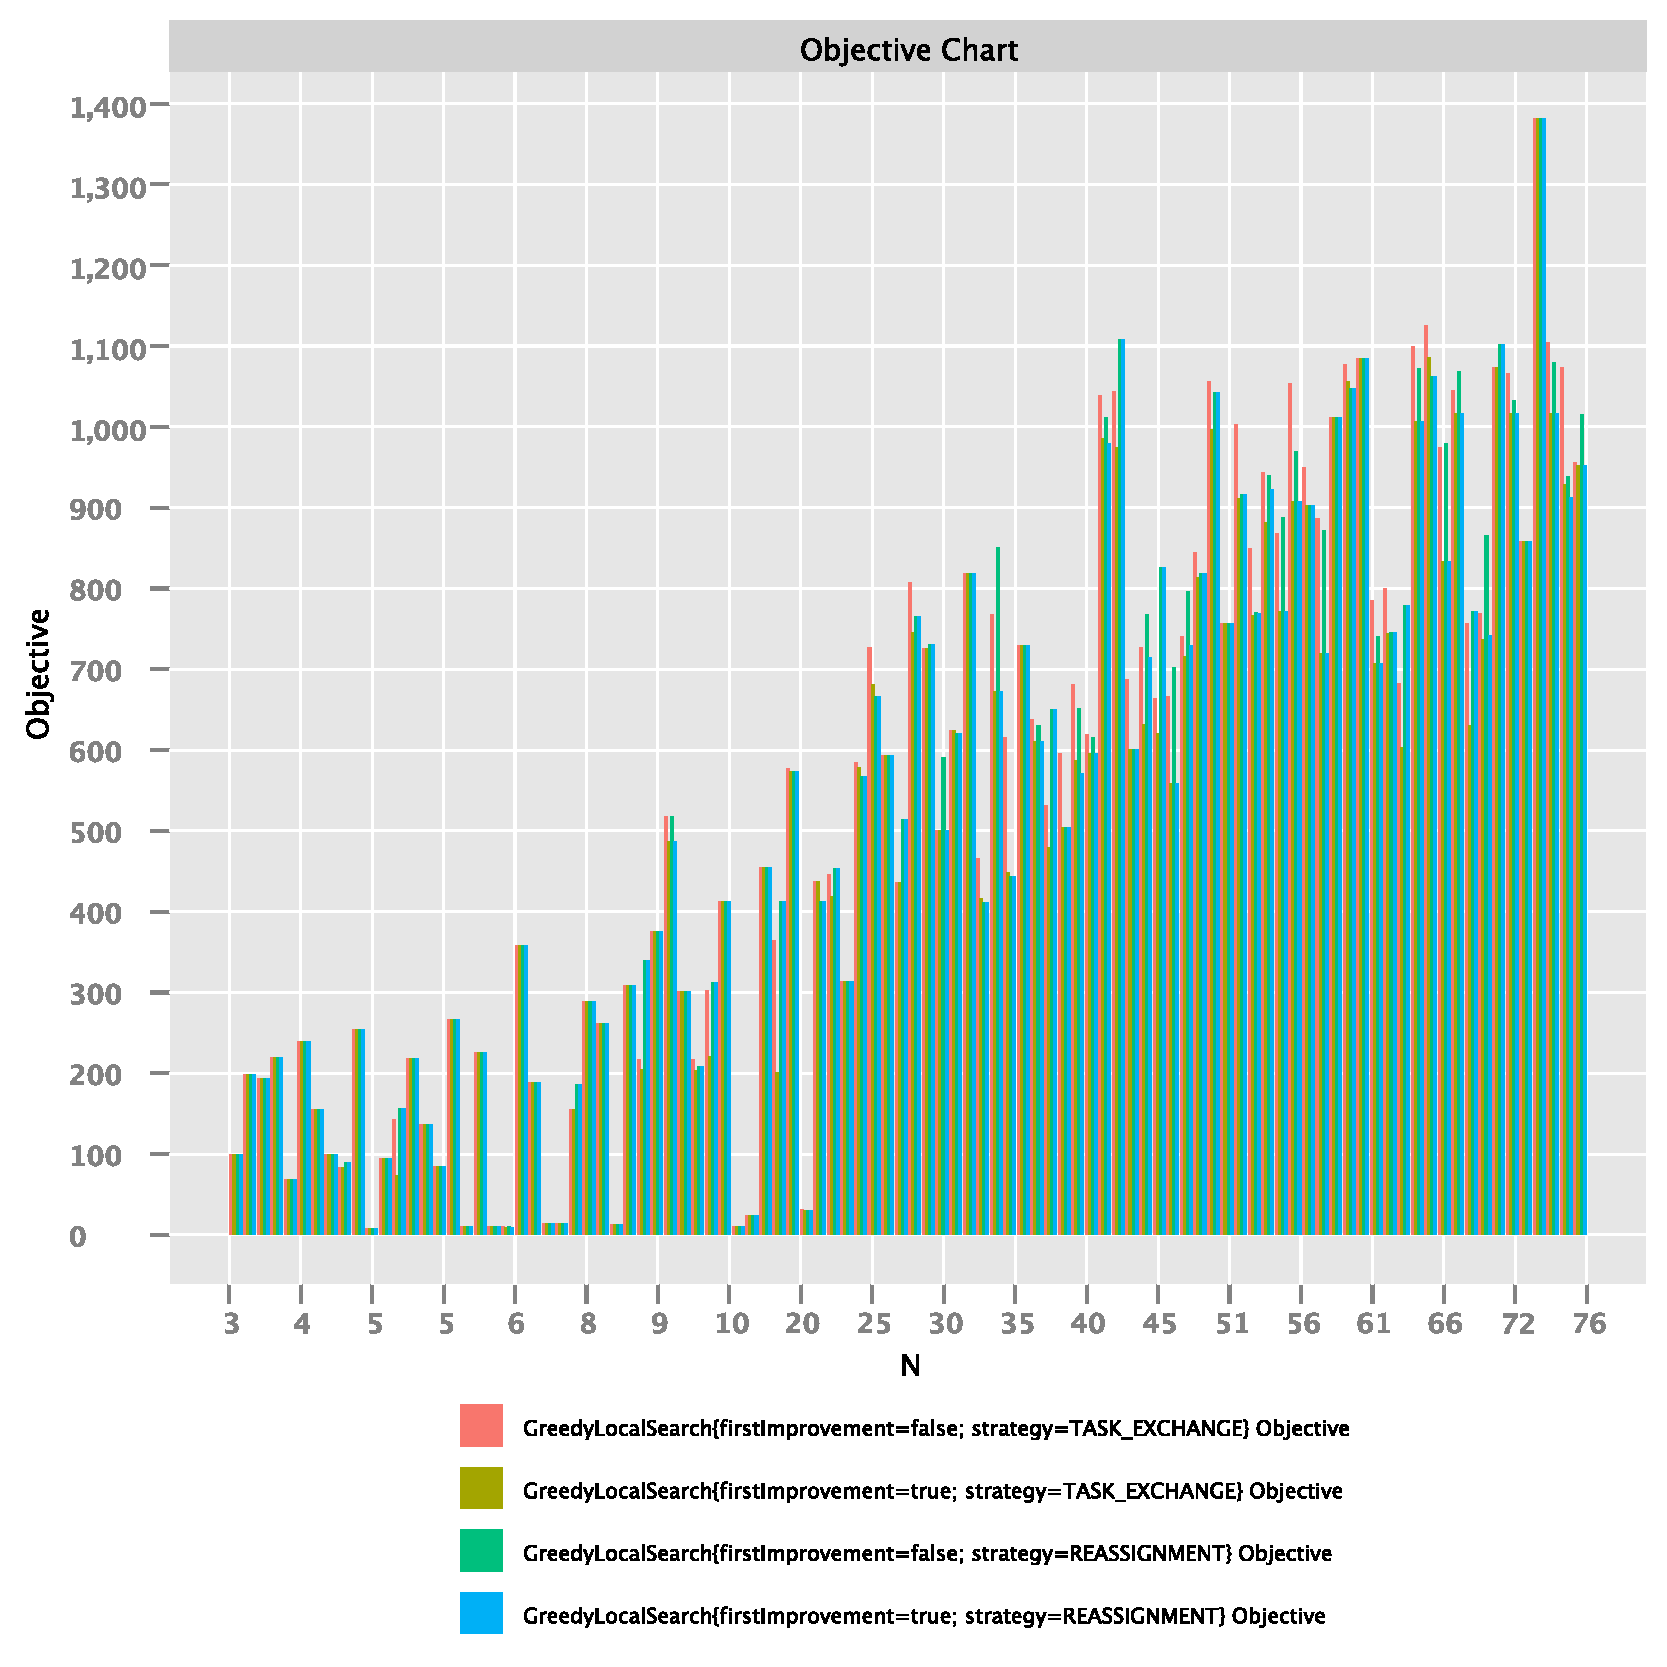
\includegraphics[width=1\textwidth]{./documentation/assets/localSearchParams.objectiveChart.pdf}
    \caption{Objective Parameters Local Search}
    \label{fig:local_time}
\end{figure}\FloatBarrier

\newpage

\section{Tuning GRASP}

\begin{figure}[!h]
    \centering
    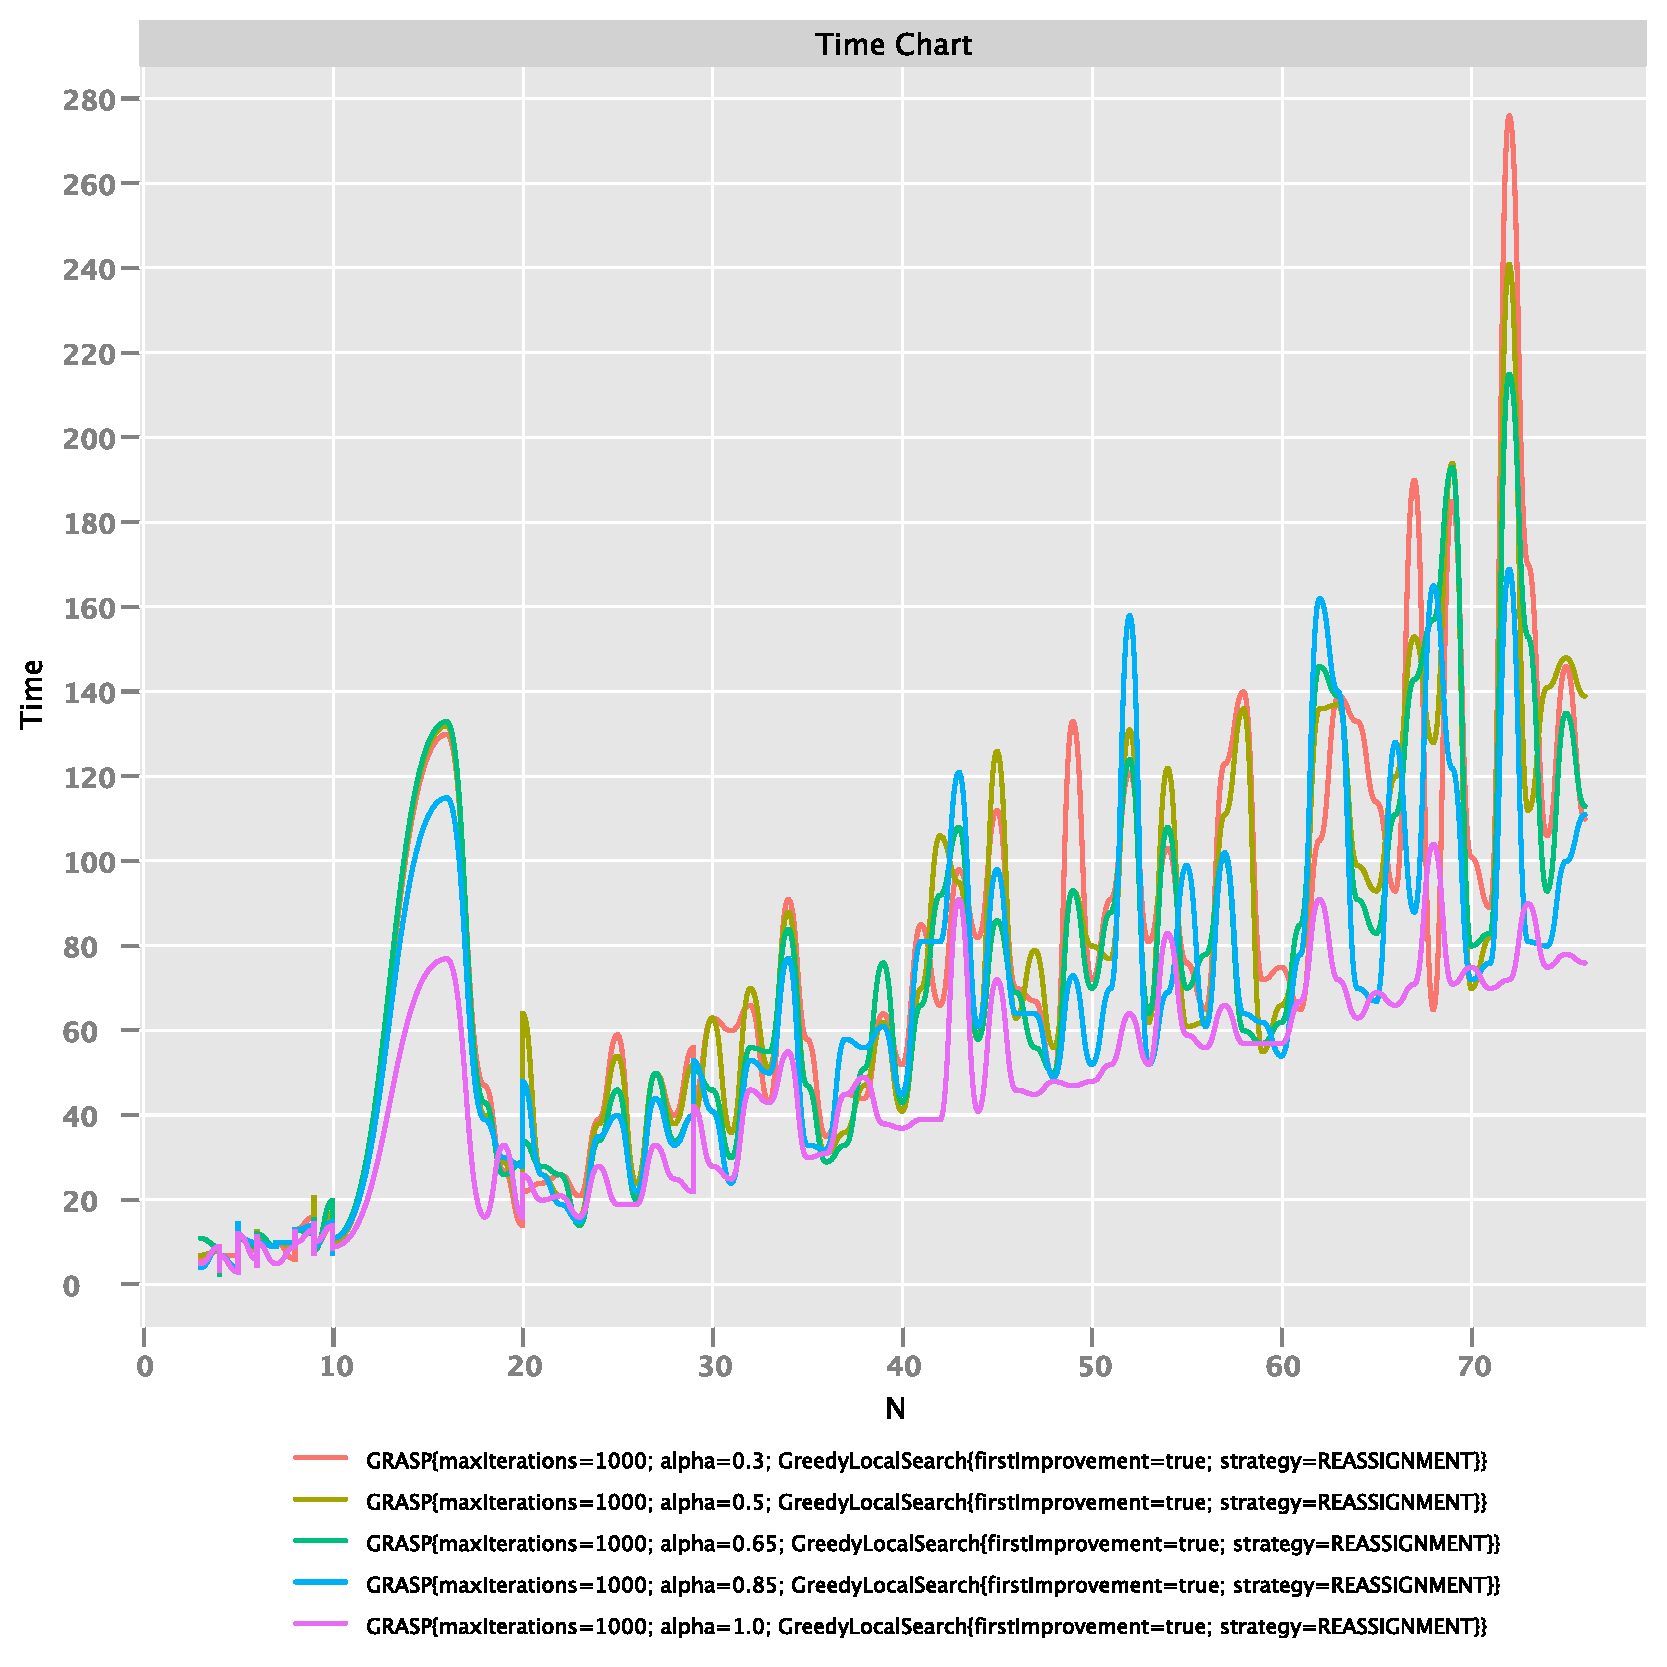
\includegraphics[width=1\textwidth]{./documentation/assets/GRASPParams.timeChart.pdf}
    \caption{Time Parameters GRASP}
    \label{fig:grasp_time}
\end{figure}\FloatBarrier

\begin{figure}
    \centering
    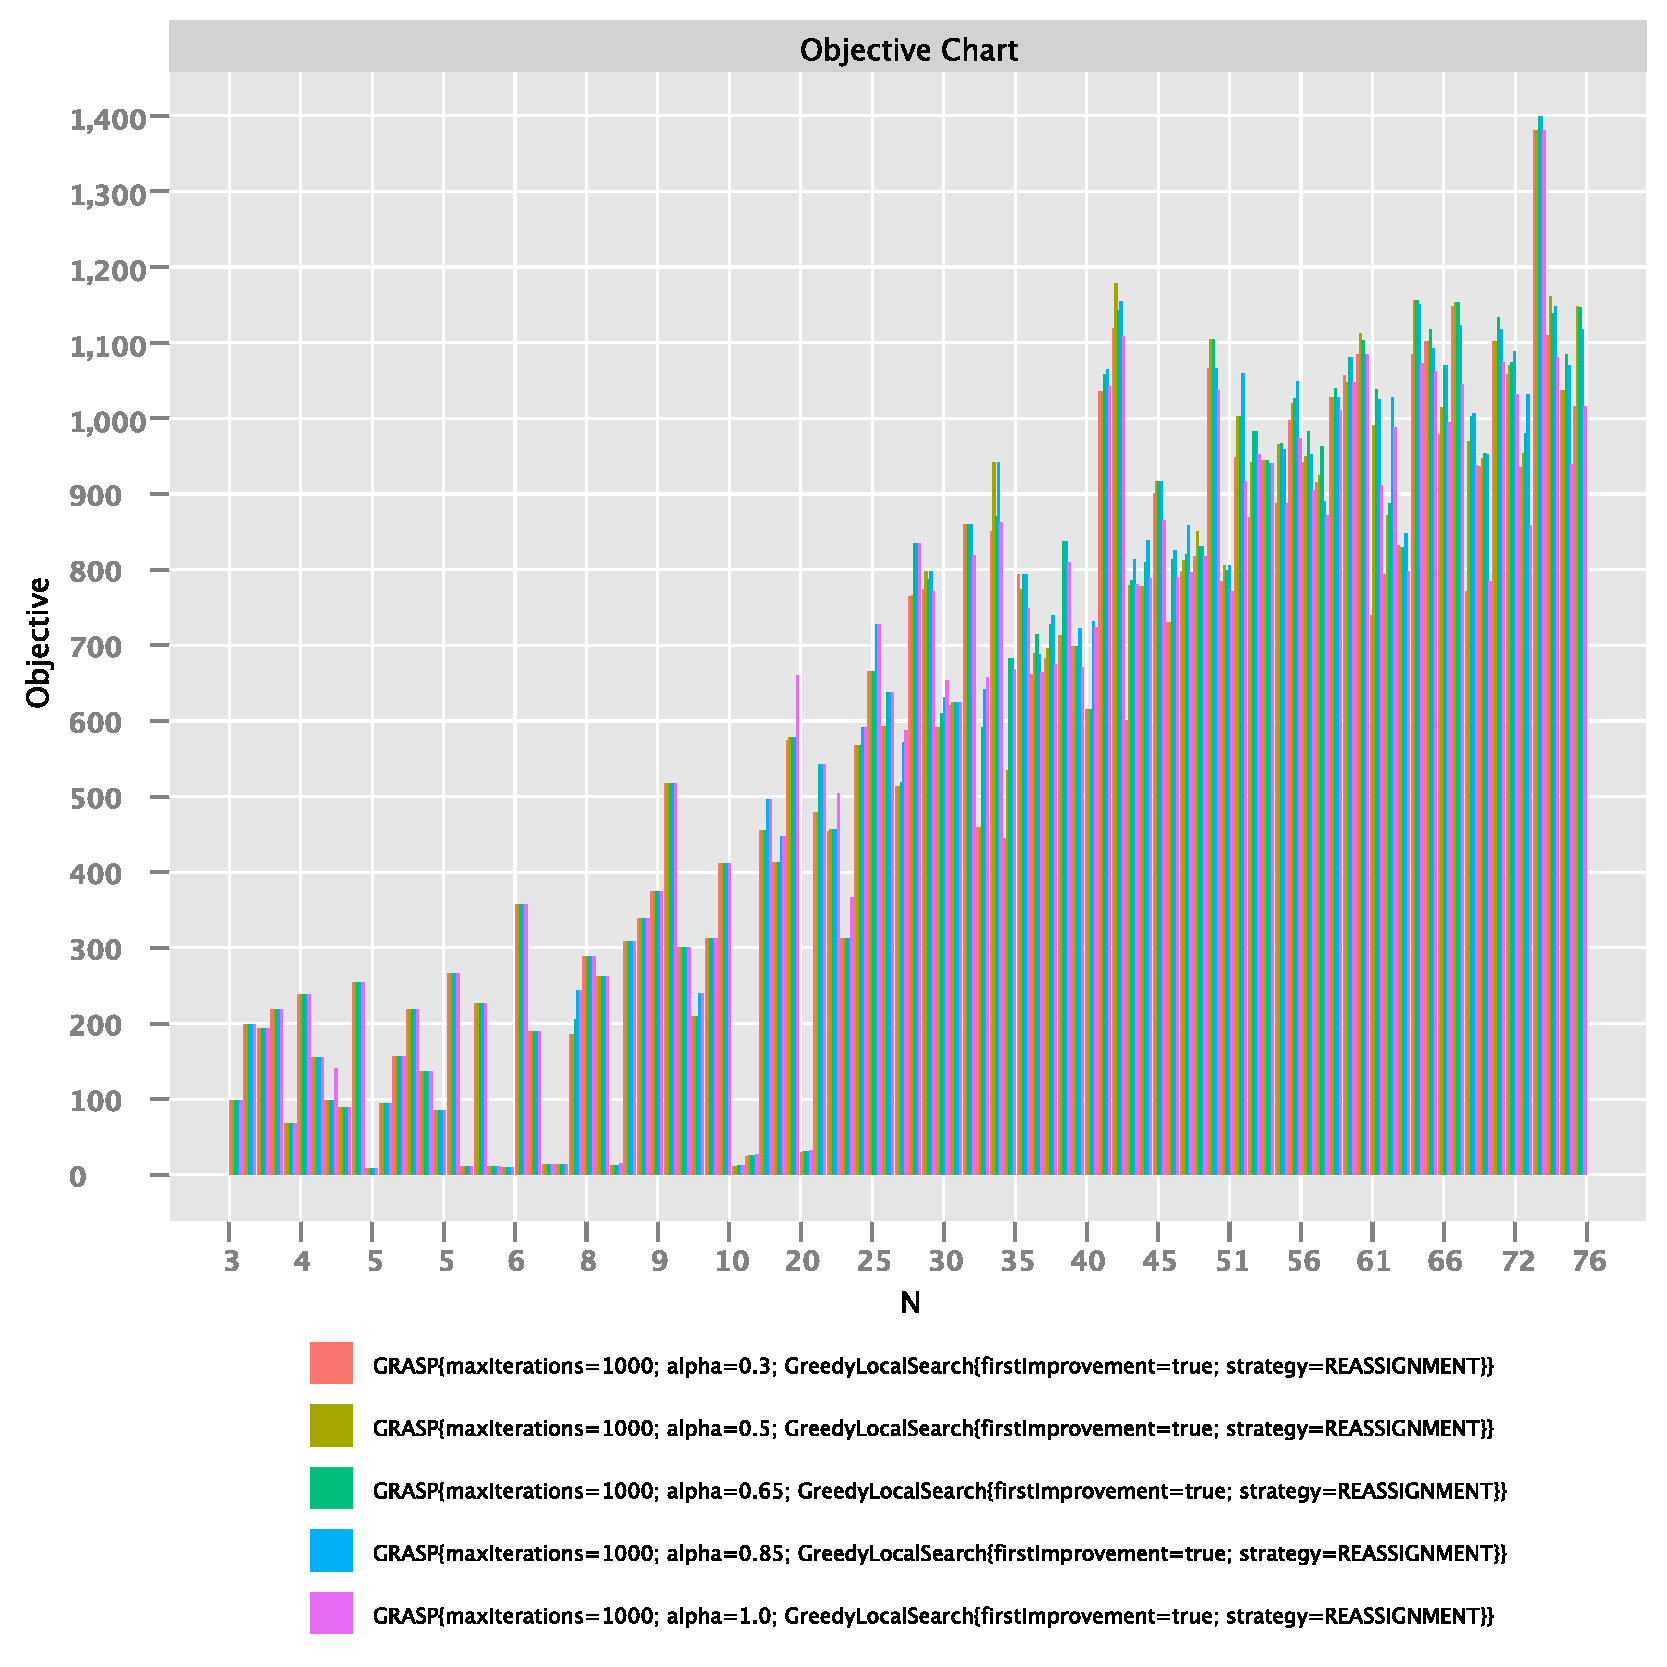
\includegraphics[width=1\textwidth]{./documentation/assets/GRASPParams.objectiveChart.pdf}
    \caption{Objective Parameters GRASP}
    \label{fig:grasp_time}
\end{figure}\FloatBarrier

\newpage

\section{Performance overall}

\begin{figure}[!h]
    \centering
    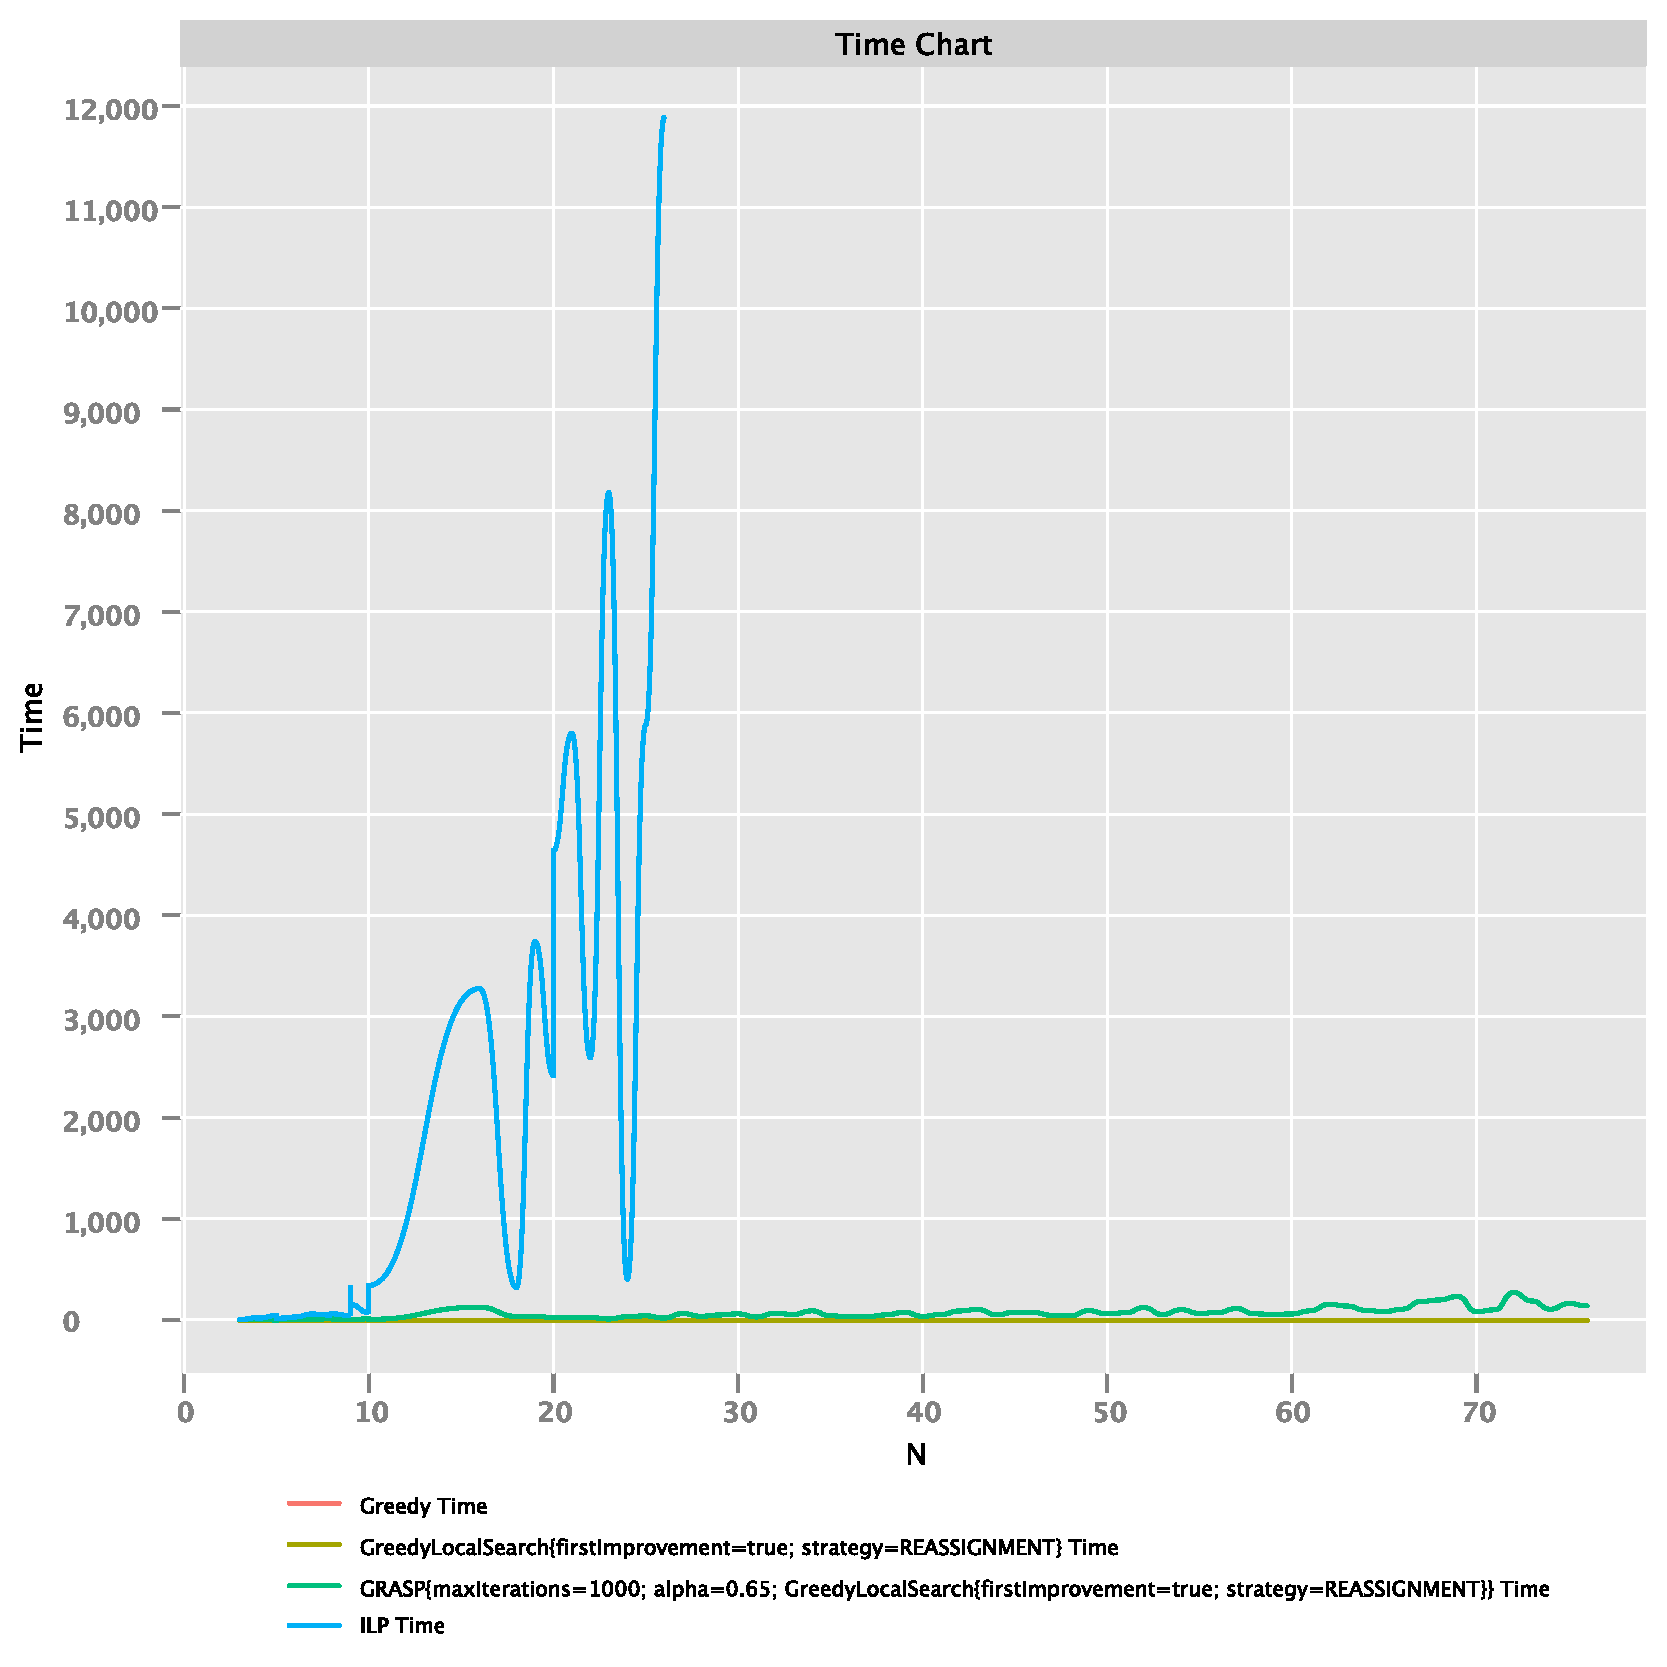
\includegraphics[width=1\textwidth]{./documentation/assets/all.timeChart.pdf}
    \caption{Time}
    \label{fig:all_time}
\end{figure}\FloatBarrier

\begin{figure}
    \centering
    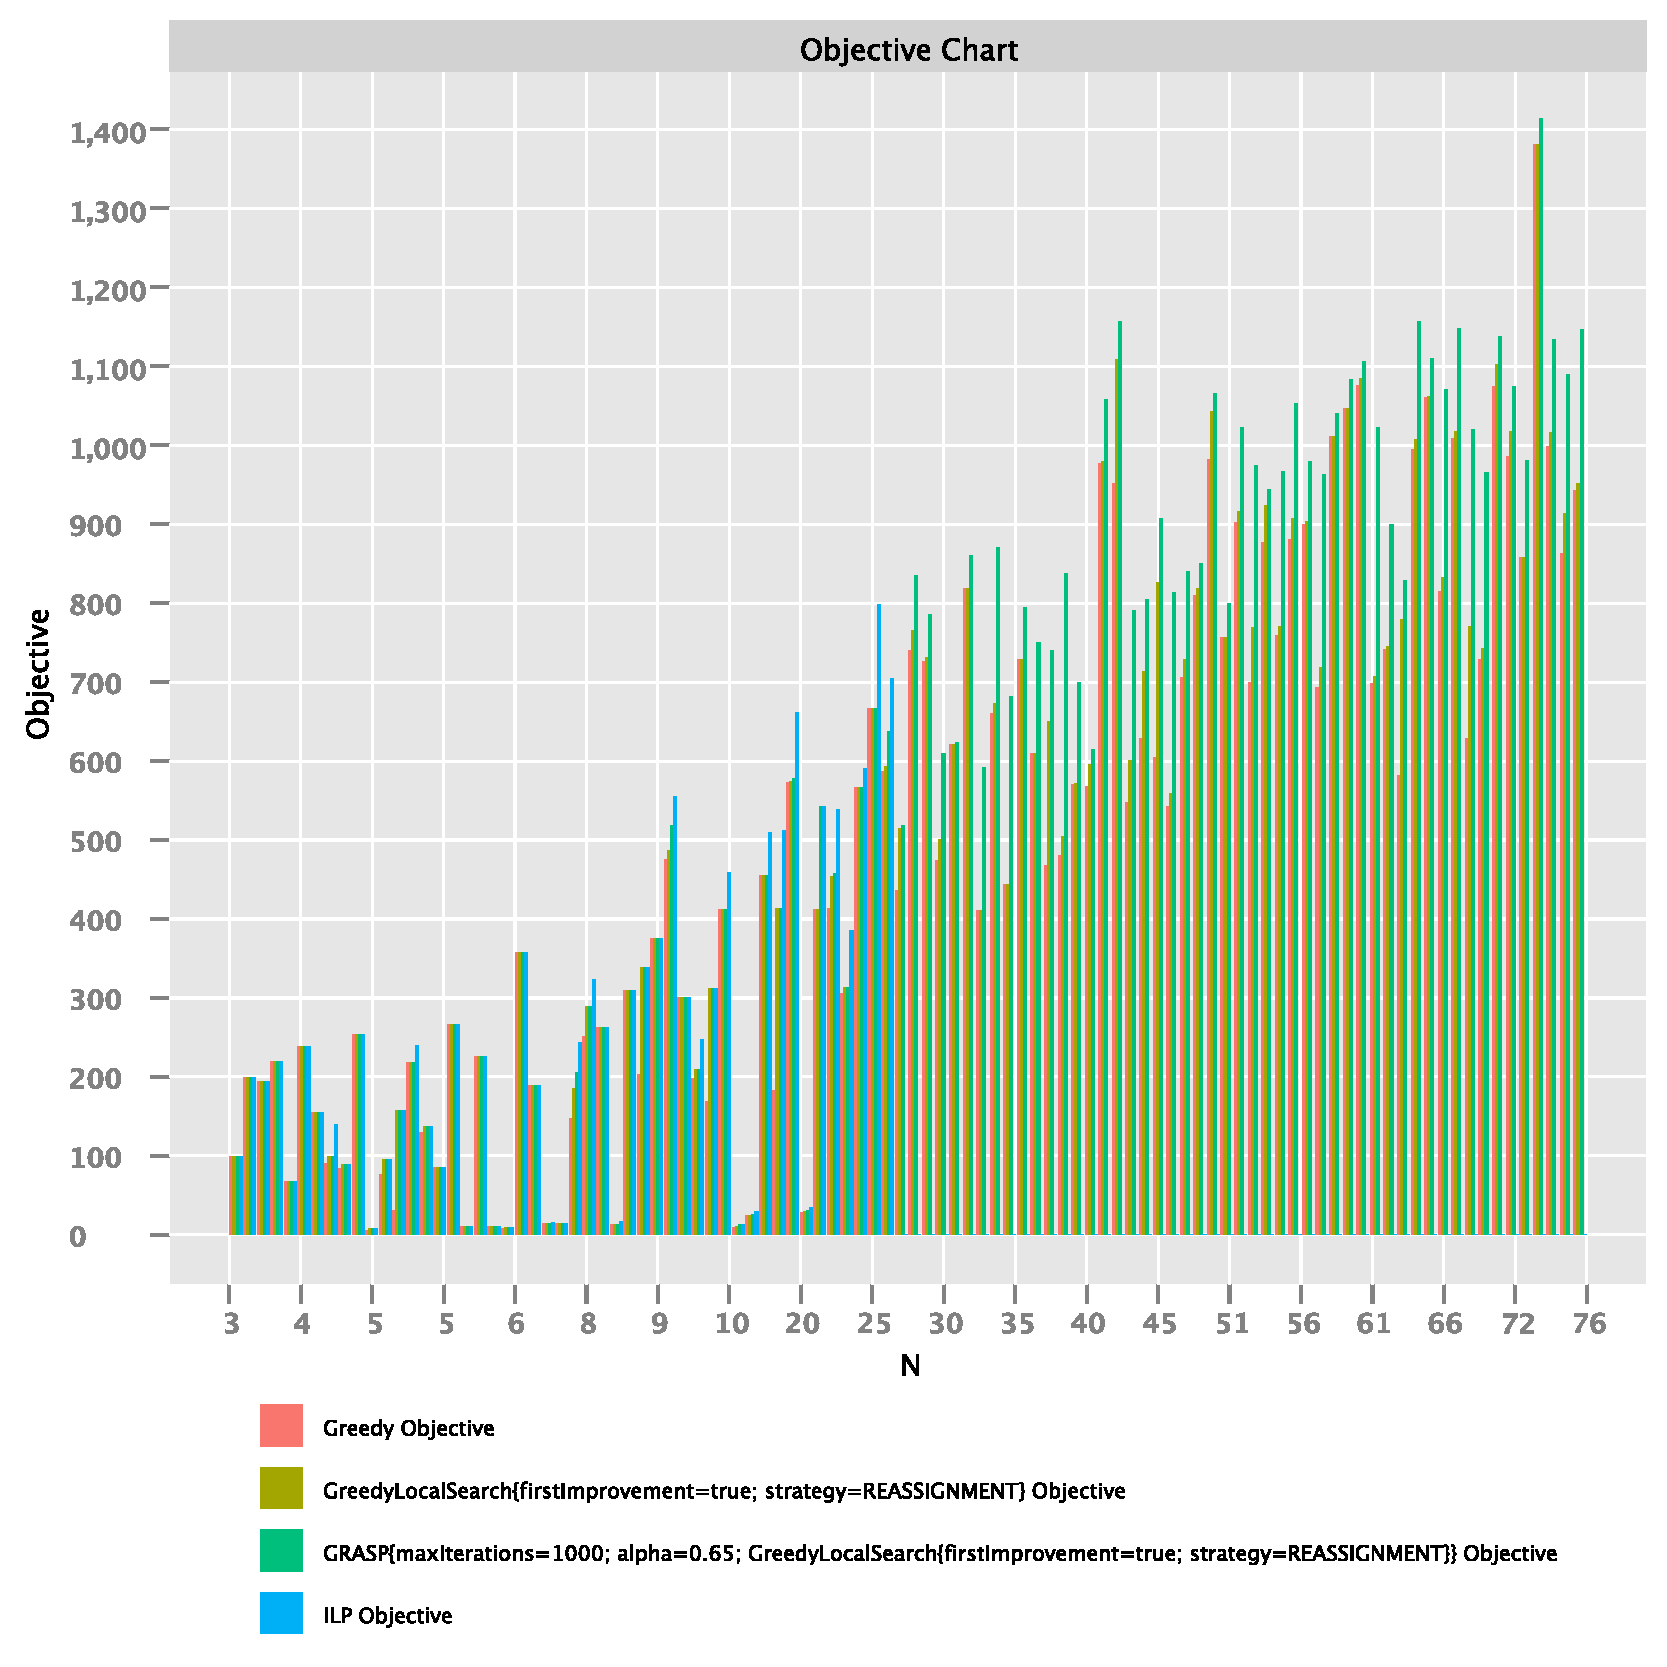
\includegraphics[width=1\textwidth]{./documentation/assets/all.objectiveChart.pdf}
    \caption{Objective}
    \label{fig:all_time}
\end{figure}\FloatBarrier

\section{How to run}

This will run both OPL and Heuristic and output benchmark values in CSV.

\begin{lstlisting}[language=bash]
cd heuristic
mvn compile exec:java -Dexec.mainClass="edu.upc.fib.ammm.Main" ../opl
\end{lstlisting}

\end{document}